\chapter{Results}\label{ch:results}

\section{The power-of-two baseline}
The simplest increment is $c=2^{-k}$. The power-of-two grid implies only three possible numerical outcomes under the assumptions of Chapter~\ref{ch:theory}: the original value $c$ is preserved when $u\le c$, the increment is absorbed when $u>2c$, or a half-way case $u=2c$ produces either $0$ or $2c$ depending on parity. This is precisely the pattern observed by the source notebook.

\begin{table}[htbp]
\centering
\caption{Classification of 780 binary64 evaluations with $x\in\{2,\ldots,40\}$ and $c=2^{-k}$ for $k\in\{1,\ldots,20\}$. Counts were independently regenerated.}\label{tab:powercount}
\begin{tabular}{lrr}
\toprule
Outcome & Condition & Cases\\
\midrule
Increment preserved, $f=c$ & $c\ge u$ & 379\\
Increment absorbed, $f=0$ & $c<u/2$ & 371\\
Half-way, rounded downward & $c=u/2$ & 28\\
Half-way, rounded upward, $f=2c$ & $c=u/2$ & 2\\
\midrule
Total &&780\\
\bottomrule
\end{tabular}
\end{table}

\begin{figure}[htbp]
\centering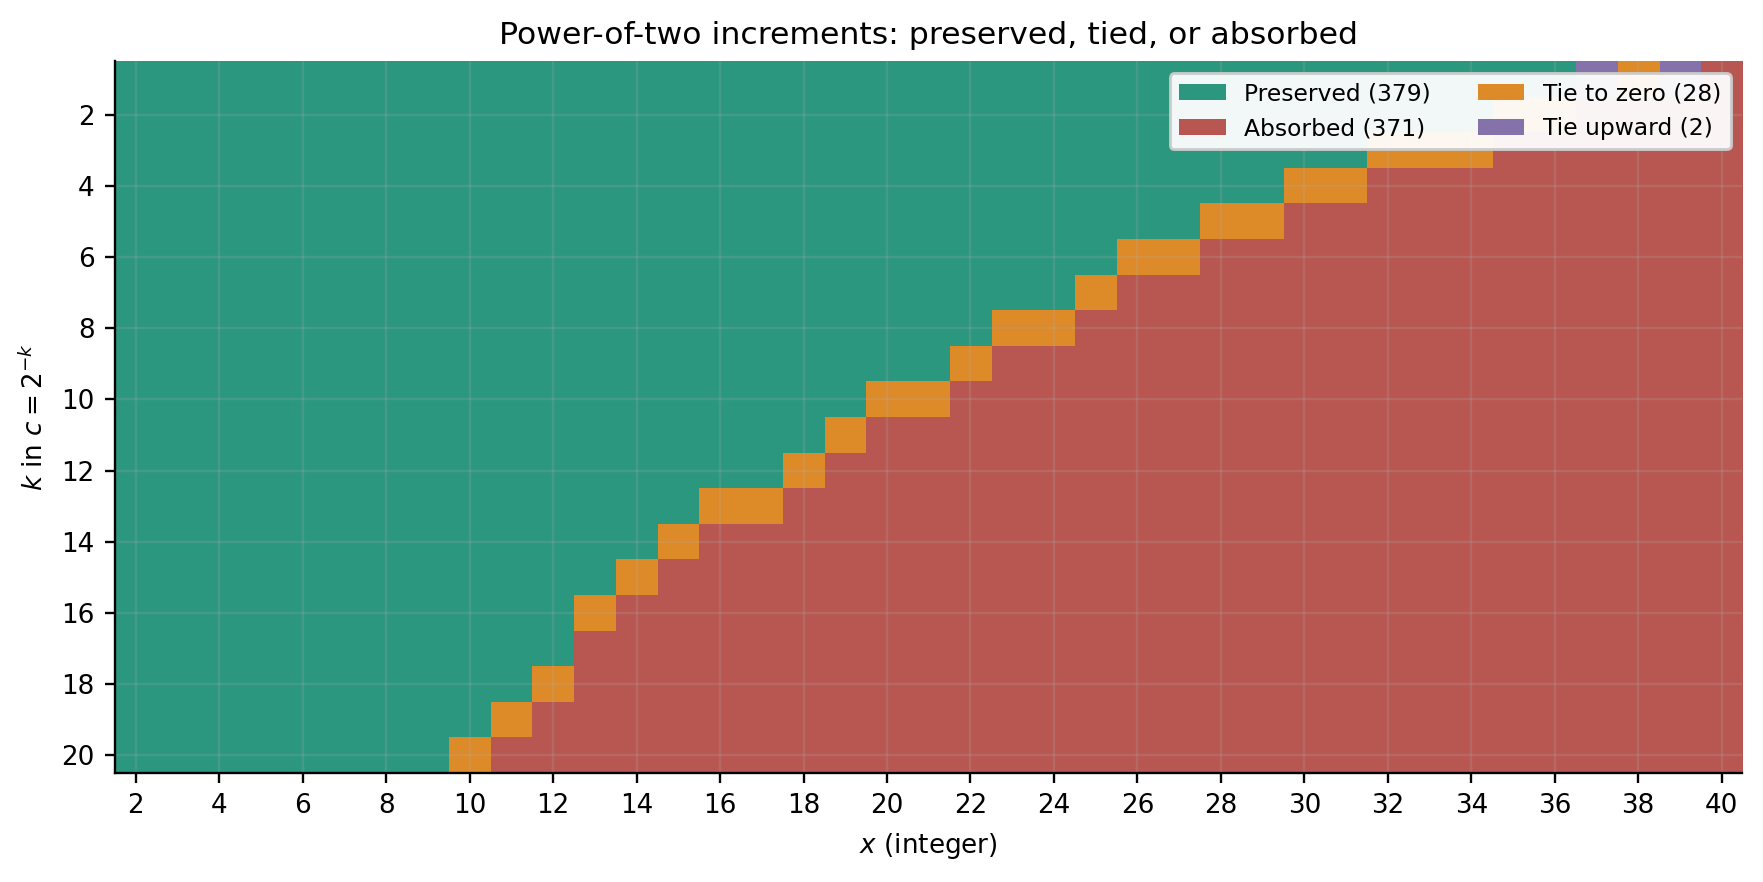
\includegraphics[width=.98\textwidth]{figs/02_power_two_map.png}
\caption{Power-of-two increment map on the 780-case integer grid. At a given $x$, smaller increments are absorbed; the narrow tie boundary separates preserved and absorbed results.}\label{fig:powmap}
\end{figure}

The 30 ties are not an implementation defect: both neighboring results are equally close to the exact sum, so ties-to-even selects according to the binary significand of $y$. Across a continuous $x$ grid, different sampled significands exhibit both possible tie outcomes. The observed transition zone for $c=2^{-1}$ is approximately $36.76\le x<39.40$; for $c=2^{-10}$ it is about $19.70\le x<21.11$, as described in the supplied preliminary report.

\begin{figure}[htbp]
\centering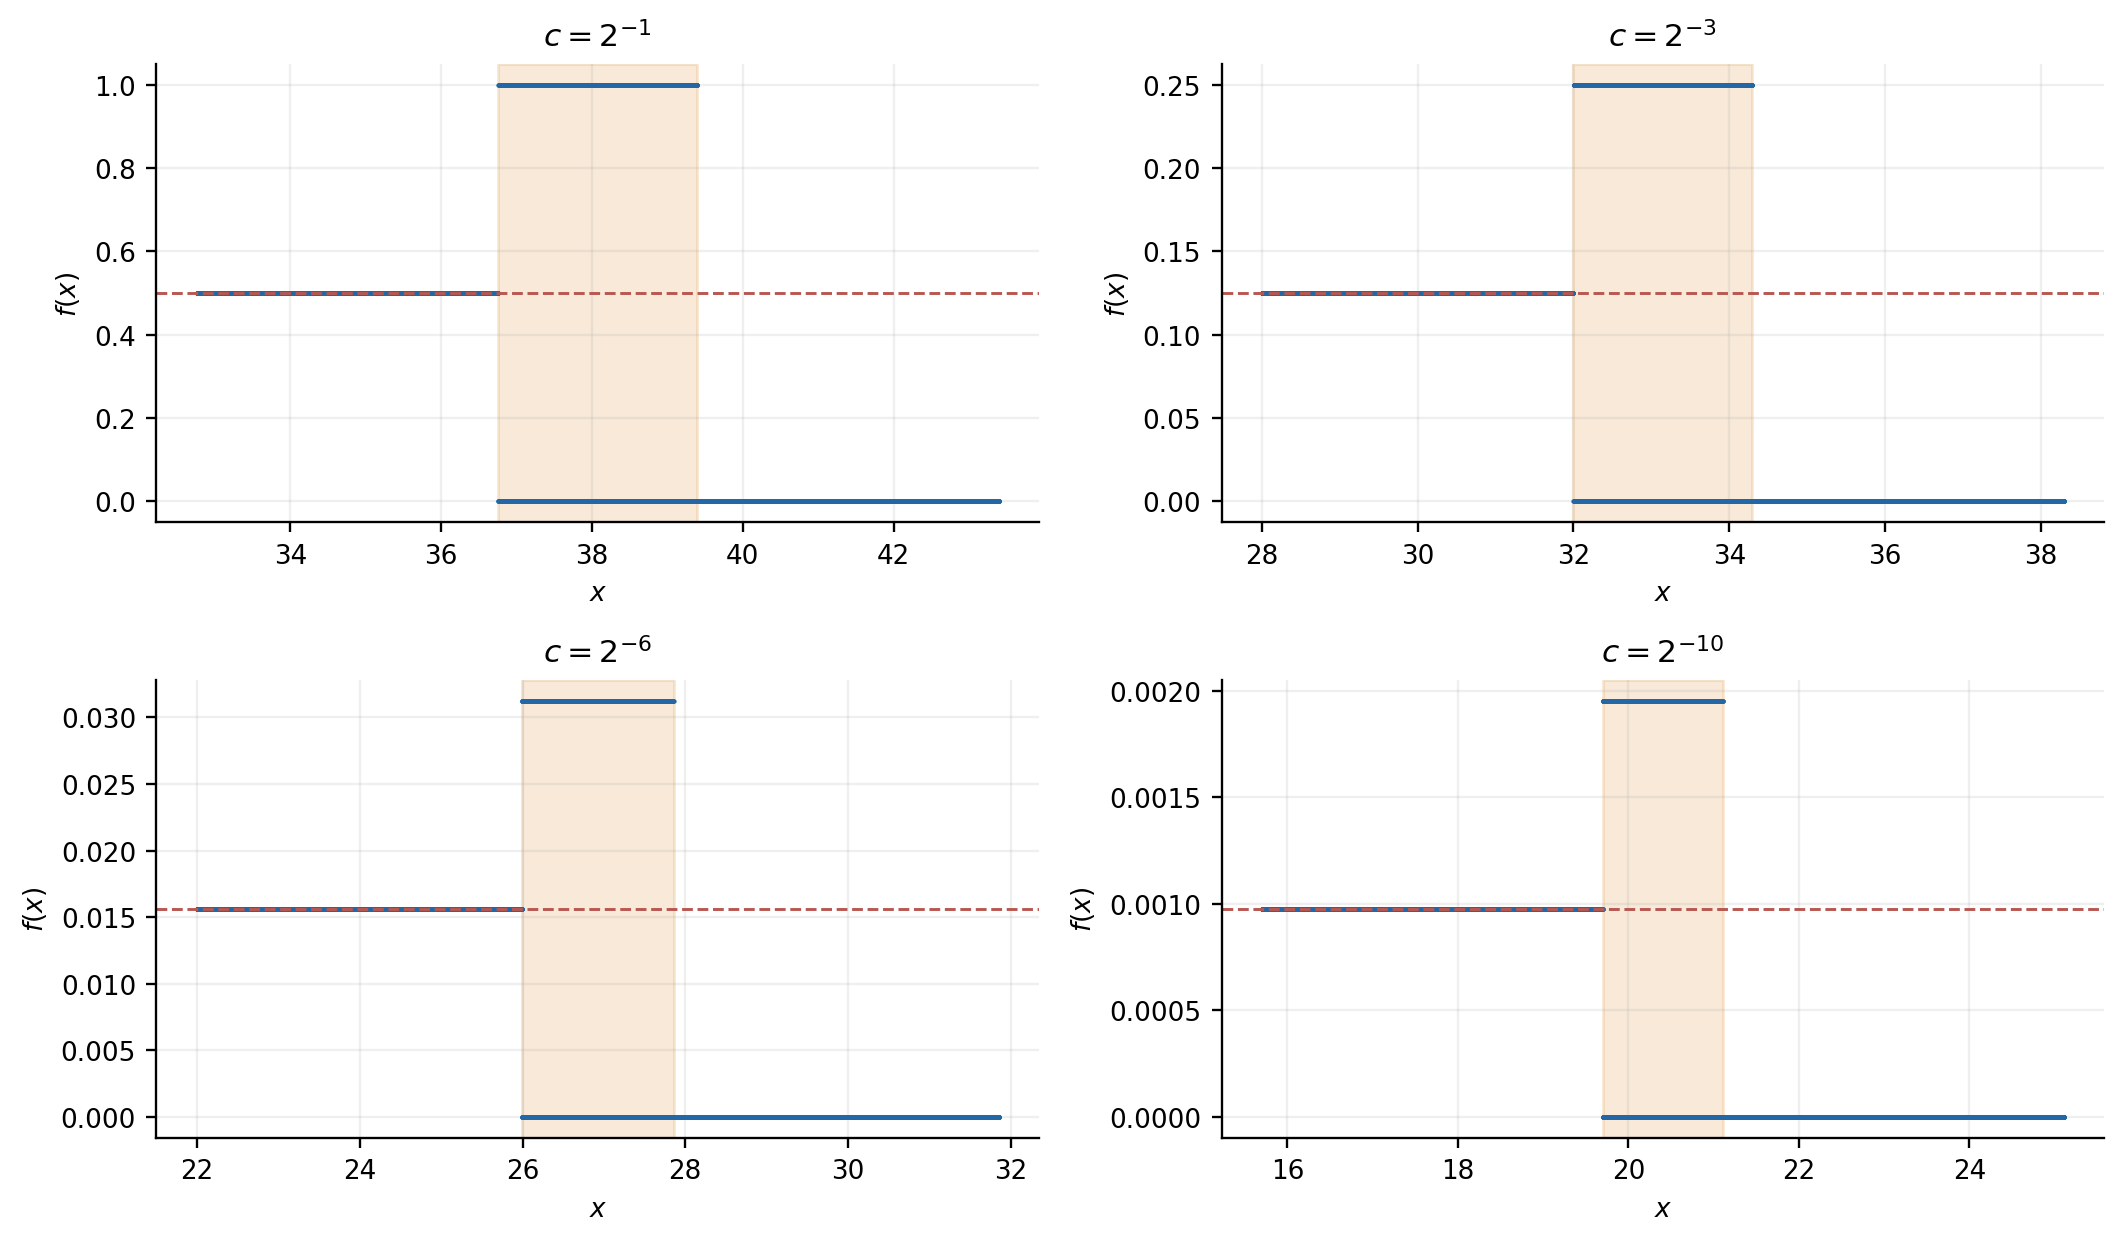
\includegraphics[width=.96\textwidth]{figs/03_power_two_curves.png}
\caption{Continuous numerical curves for $c=2^{-1},2^{-3},2^{-6},2^{-10}$ (binary64), corresponding to the supplied continuous Plotly experiments. The shaded strip identifies the parity-sensitive binade.}\label{fig:powcurves}
\end{figure}

\section{Odd integer increments}
For every positive odd integer $c$ representable in the chosen precision, $\nu(c)=0$. Therefore the onset of inexactness, when $y\ge c$ and binade crossing is excluded, does not depend on the \emph{value} of $c$: the first affected binade is $E=p$. For binary64 this begins near $x_1\approx39.40$, while for binary32 it begins near $x_1\approx5.28$. The end of the inexact zone does depend on the size of $c$ through $\lambda=\lfloor\log_2c\rfloor$.

\begin{table}[htbp]
\centering
\caption{Predicted first inexact and fully absorbed boundaries for selected positive odd integers, binary64. Values are rounded to two decimal places.}\label{tab:oddthreshold}
\begin{tabular}{rrrr}
\toprule
$c$ & $L$ (binades) & $x_1$ & $x_2$\\
\midrule
$1$ & 1 &39.40&42.22\\
$3$ & 2 &39.40&45.25\\
$5$ or $7$ &3&39.40&48.50\\
$21$&5&39.40&55.72\\
$101$&7&39.40&64.00\\
$1001$&10&39.40&78.79\\
$65537$&17&39.40&128.00\\
\bottomrule
\end{tabular}
\end{table}

At the first inexact binade, $u=2$ and every odd integer $c$ lies halfway between two multiples of two. The output is therefore $c-1$ or $c+1$. For all later interior binades, $u=4,8,16,\ldots$ and the computed increment changes by discrete jumps. In this regime $f$ is not necessarily monotonic in $x$; it can move above and below the exact value as different low-order bits of $c$ are discarded.

\begin{figure}[htbp]
\centering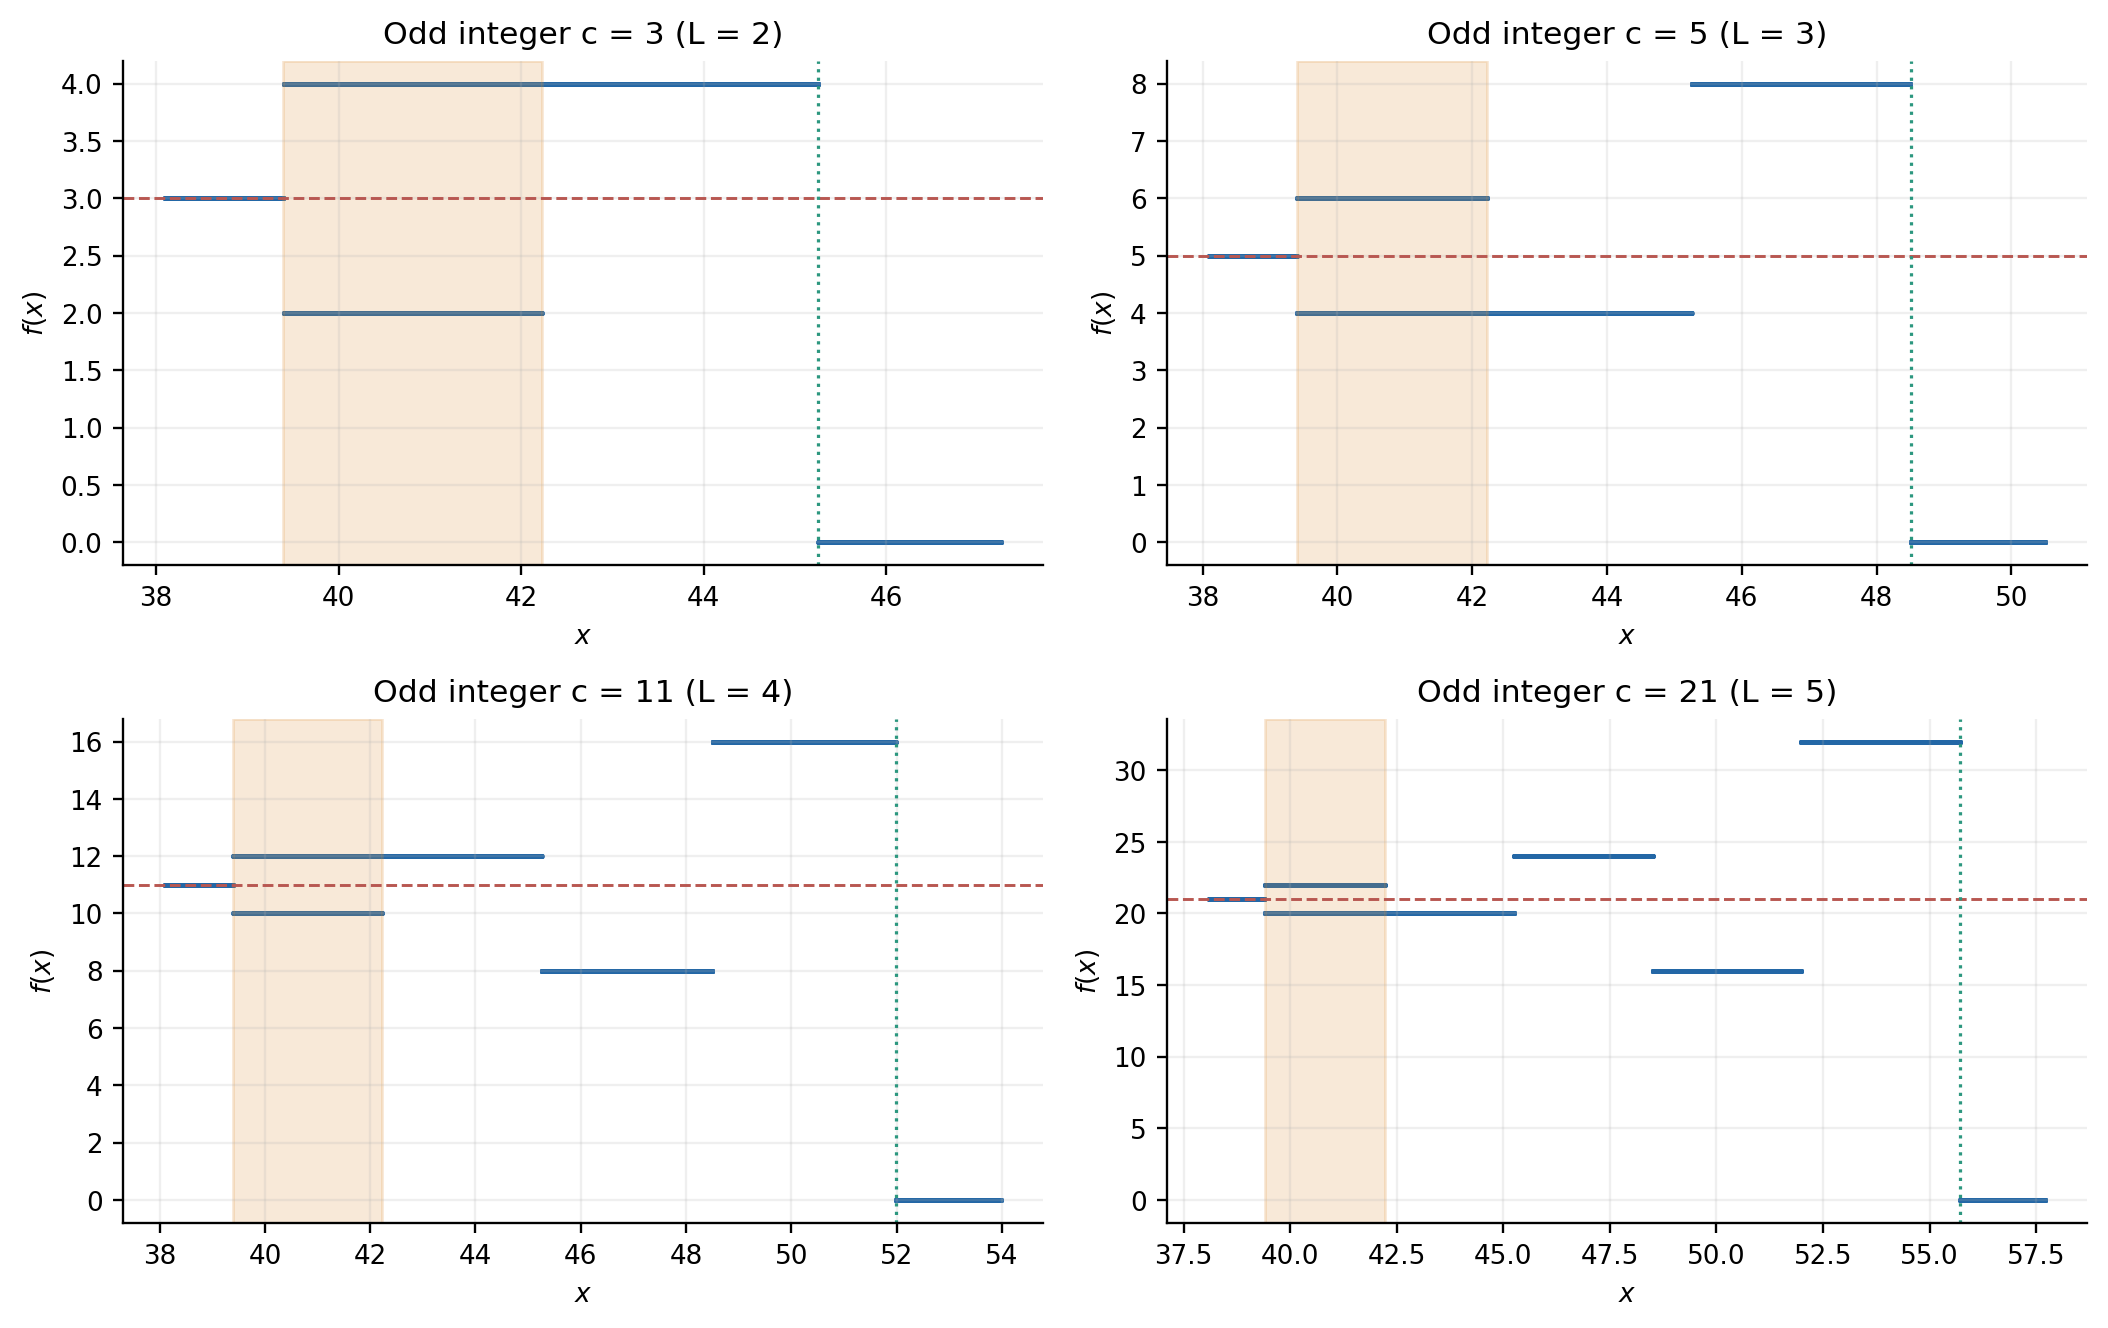
\includegraphics[width=.96\textwidth]{figs/04_odd_integer_curves.png}
\caption{Odd-integer experiments ($c=3,5,11,21$) reconstructed in English from the supplied family of Plotly curves. Dashed horizontal lines show the exact increment; dotted vertical lines mark the predicted complete-absorption boundaries.}\label{fig:oddcurves}
\end{figure}

For example, the manuscript presents $c=101$ as a particularly informative case. The output is $100$ or $102$ at $u=2$, then $100$ at $u=4$, $104$ at $u=8$, $96$ at $u=16$ and $u=32$, $128$ at $u=64$ and $u=128$, and $0$ from $u=256$ onward. The result $128$ represents a relative error $(128-101)/101\approx26.7\%$, despite being less than half of the ULP of $y$ in the relevant binade.

\begin{table}[htbp]
\centering\small
\caption{Model values for $c=101$ in binary64, taken from the supplied study. The tie binade has two possible values.}\label{tab:odd101}
\begin{tabular}{r r l r}
\toprule
Exponent $E$ & $u$ & Computed $f$ & Normalized error $\varepsilon$\\
\midrule
$E<53$ & $\le1$ & $101$ & $0$\\
$53$ & $2$ & $100$ or $102$ & $-0.5$ or $+0.5$\\
$54$ & $4$ & $100$ & $-0.25$\\
$55$ & $8$ & $104$ & $+0.375$\\
$56$ & $16$ & $96$ & $-0.3125$\\
$57$ & $32$ & $96$ & $-0.15625$\\
$58$ & $64$ & $128$ & $+0.421875$\\
$59$ & $128$ & $128$ & $+0.2109375$\\
$E\ge60$ & $\ge256$ & $0$ & $\le0$\\
\bottomrule
\end{tabular}
\end{table}

The heatmap in Figure~\ref{fig:oddheatmap} summarizes odd values from $1$ to $255$. Horizontal bands arise because $x_2(c)$ changes only when $c$ crosses a power of two, while the universal onset $x_1$ remains fixed. The drawn line gives the formula for the absorption threshold, not an independent fitted boundary.

\begin{figure}[htbp]
\centering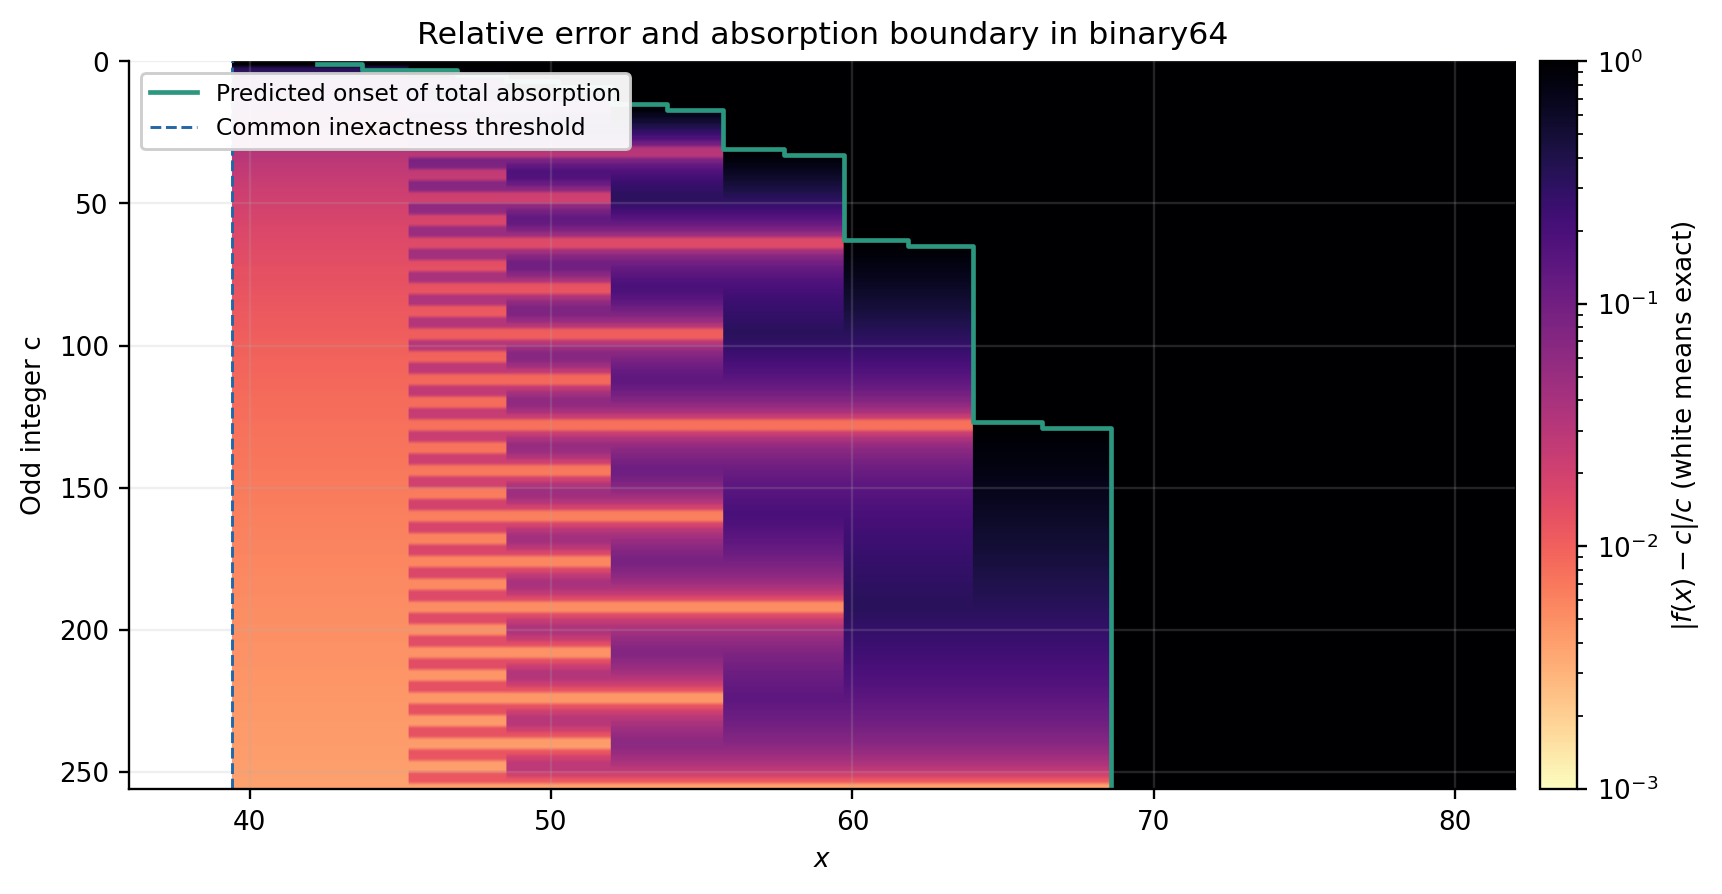
\includegraphics[width=.98\textwidth]{figs/05_odd_integer_heatmap.png}
\caption{Odd-integer relative error over a dense binary64 grid. The predicted complete-absorption boundary is superimposed on the numerical results.}\label{fig:oddheatmap}
\end{figure}

\section{Dyadic and non-dyadic fractional inputs}
Fractions of the form $m/2^j$ with odd $m$ are dyadic. Their first inexact binade is shifted by $j$ exponents compared with the same odd numerator: $\nu=-j$. Their width is still $L=\operatorname{bitlength}(m)$. For example, $c=3/4$ begins to round near $x_1\approx34.30$ and is fully absorbed from $x_2\approx39.40$; $c=5/16$ begins near $29.86$ and is fully absorbed from $36.76$.

An input such as decimal $0.1$ or mathematical $1/3$ is not dyadic. The value actually stored in a binary computer is a finite dyadic approximation and generally has many nonzero significand bits. For binary64, the stored value nearest decimal $0.1$ is $3602879701896397/2^{55}$, giving $\nu=-55$ and $L=52$. For the stored binary64 approximation to $1/3$, $L=53$. These large bit lengths imply a much longer region of affected binades than the power-of-two case.

\begin{table}[htbp]
\centering
\caption{Predicted inexact intervals for representative fractional increments. Inputs $0.1$ and $1/3$ denote their respective values after conversion to the indicated precision.}\label{tab:fractions}
\begin{tabular}{l rrr rrr}
\toprule
&\multicolumn{3}{c}{binary64}&\multicolumn{3}{c}{binary32}\\
\cmidrule(lr){2-4}\cmidrule(lr){5-7}
$c$ & $x_1$ &$x_2$ &$L$ & $x_1$ &$x_2$ &$L$\\
\midrule
$1/2$ &36.76&39.40&1&4.92&5.28&1\\
$3/4$ &34.30&39.40&2&4.59&5.28&2\\
$5/16$ &29.86&36.76&3&4.00&4.92&3\\
$0.1$ &0.87&32.00&52&0.81&4.29&24\\
$1/3$ &0.93&36.76&53&0.93&4.92&24\\
\bottomrule
\end{tabular}
\end{table}

\begin{figure}[htbp]
\centering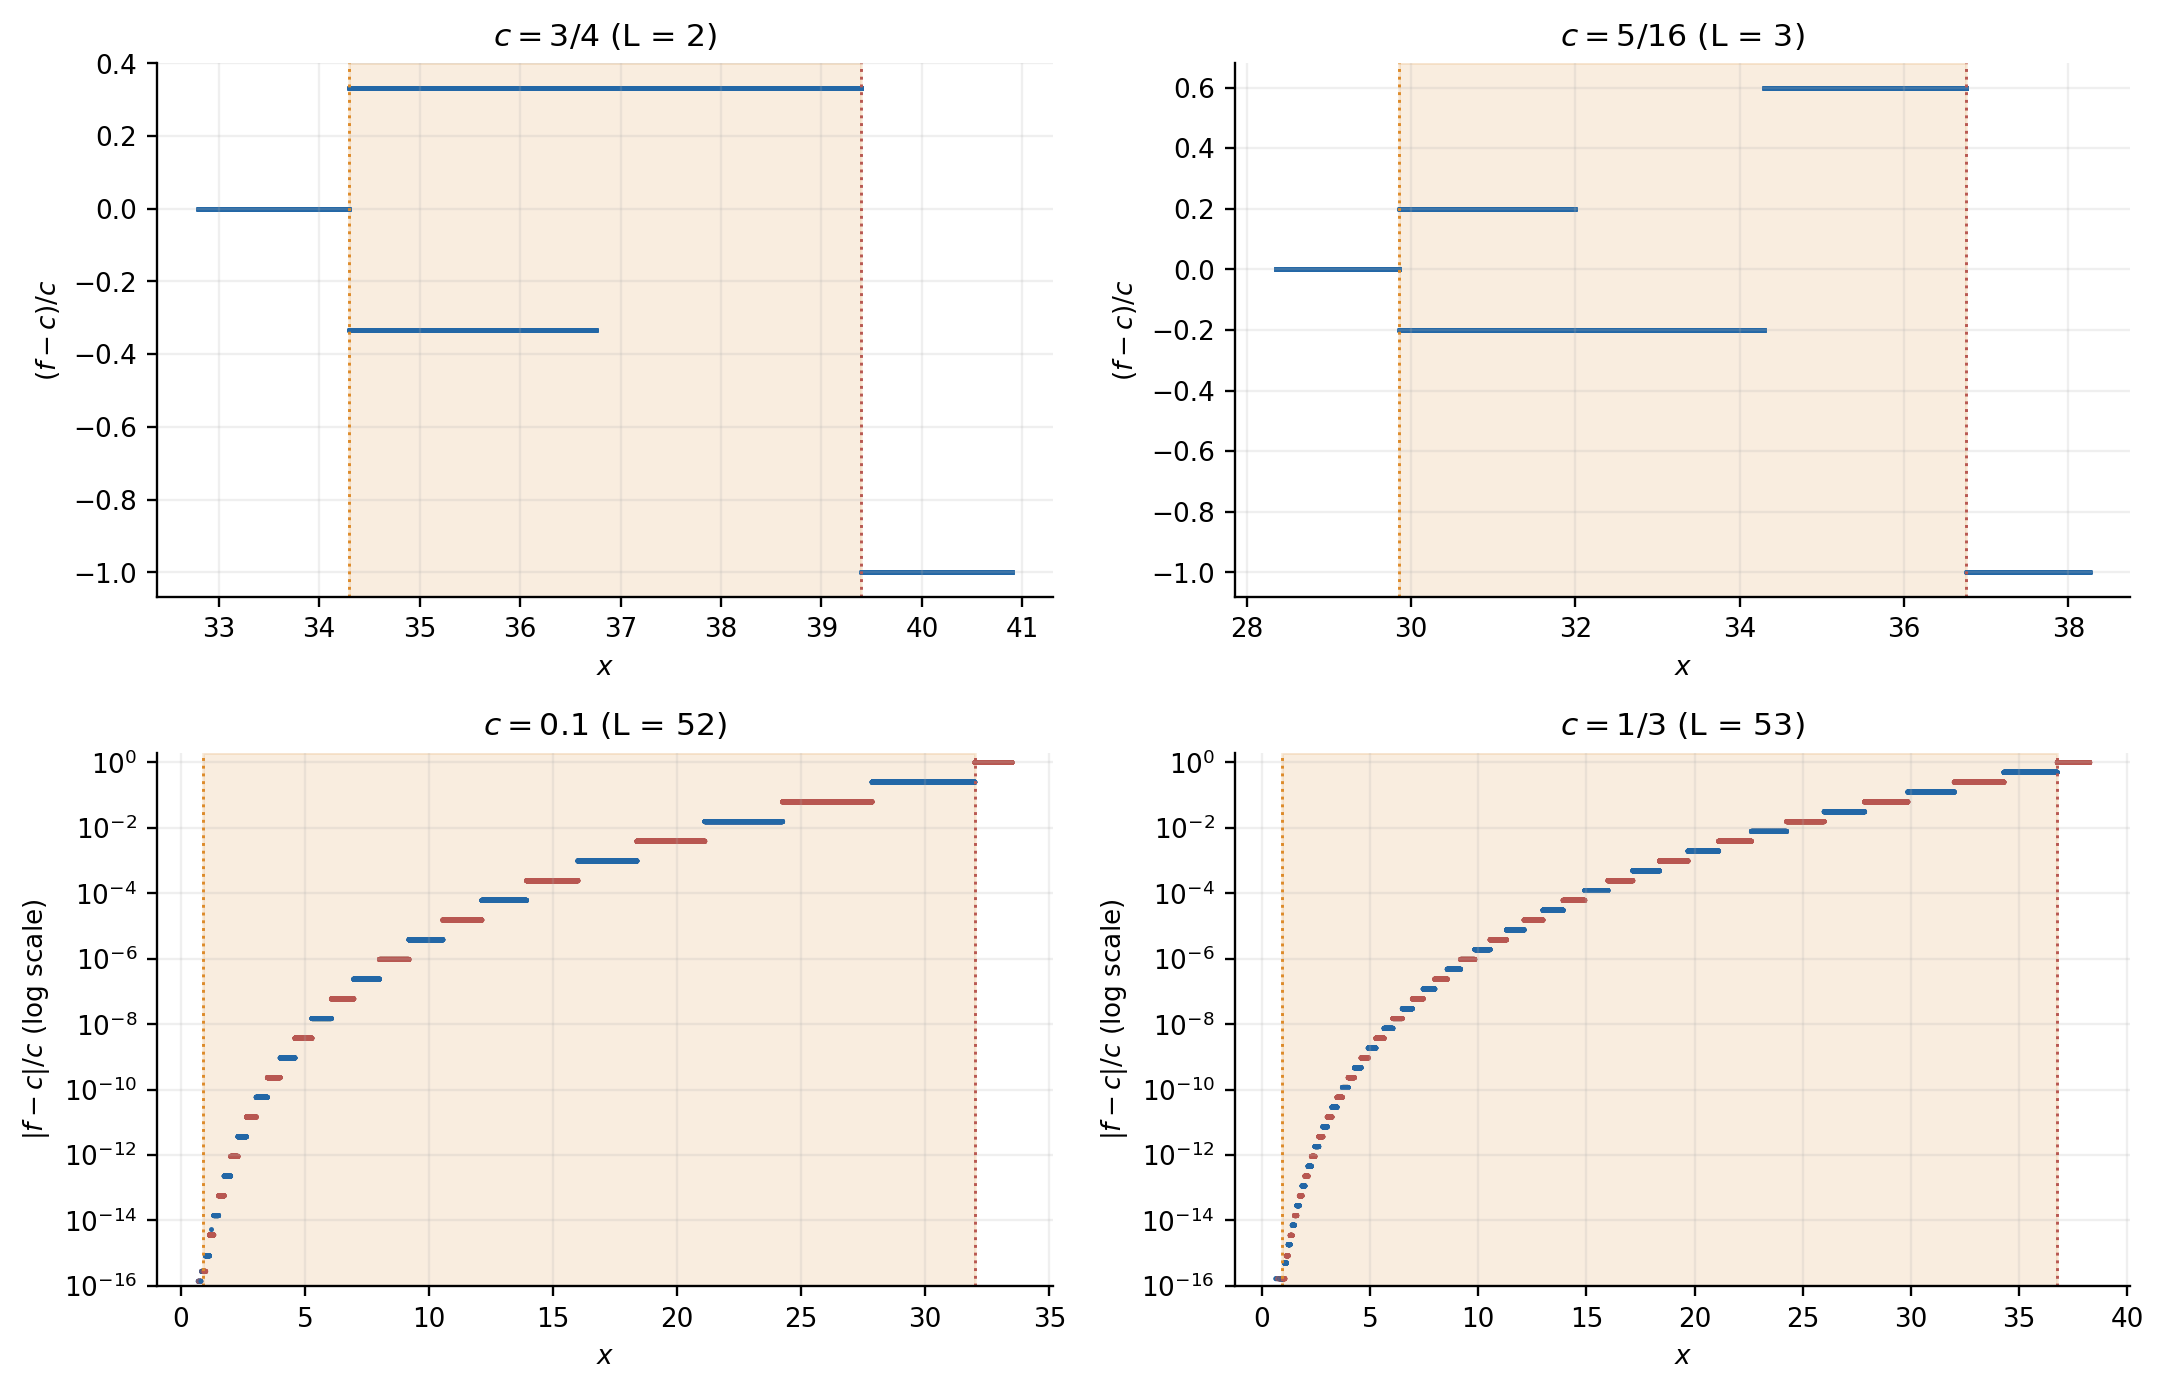
\includegraphics[width=.97\textwidth]{figs/06_fraction_behaviour.png}
\caption{Dyadic versus non-dyadic fractional increments in binary64. The lower panels show absolute relative error on a logarithmic vertical scale, exposing rounding long before absorption.}\label{fig:fractions}
\end{figure}

\begin{figure}[htbp]
\centering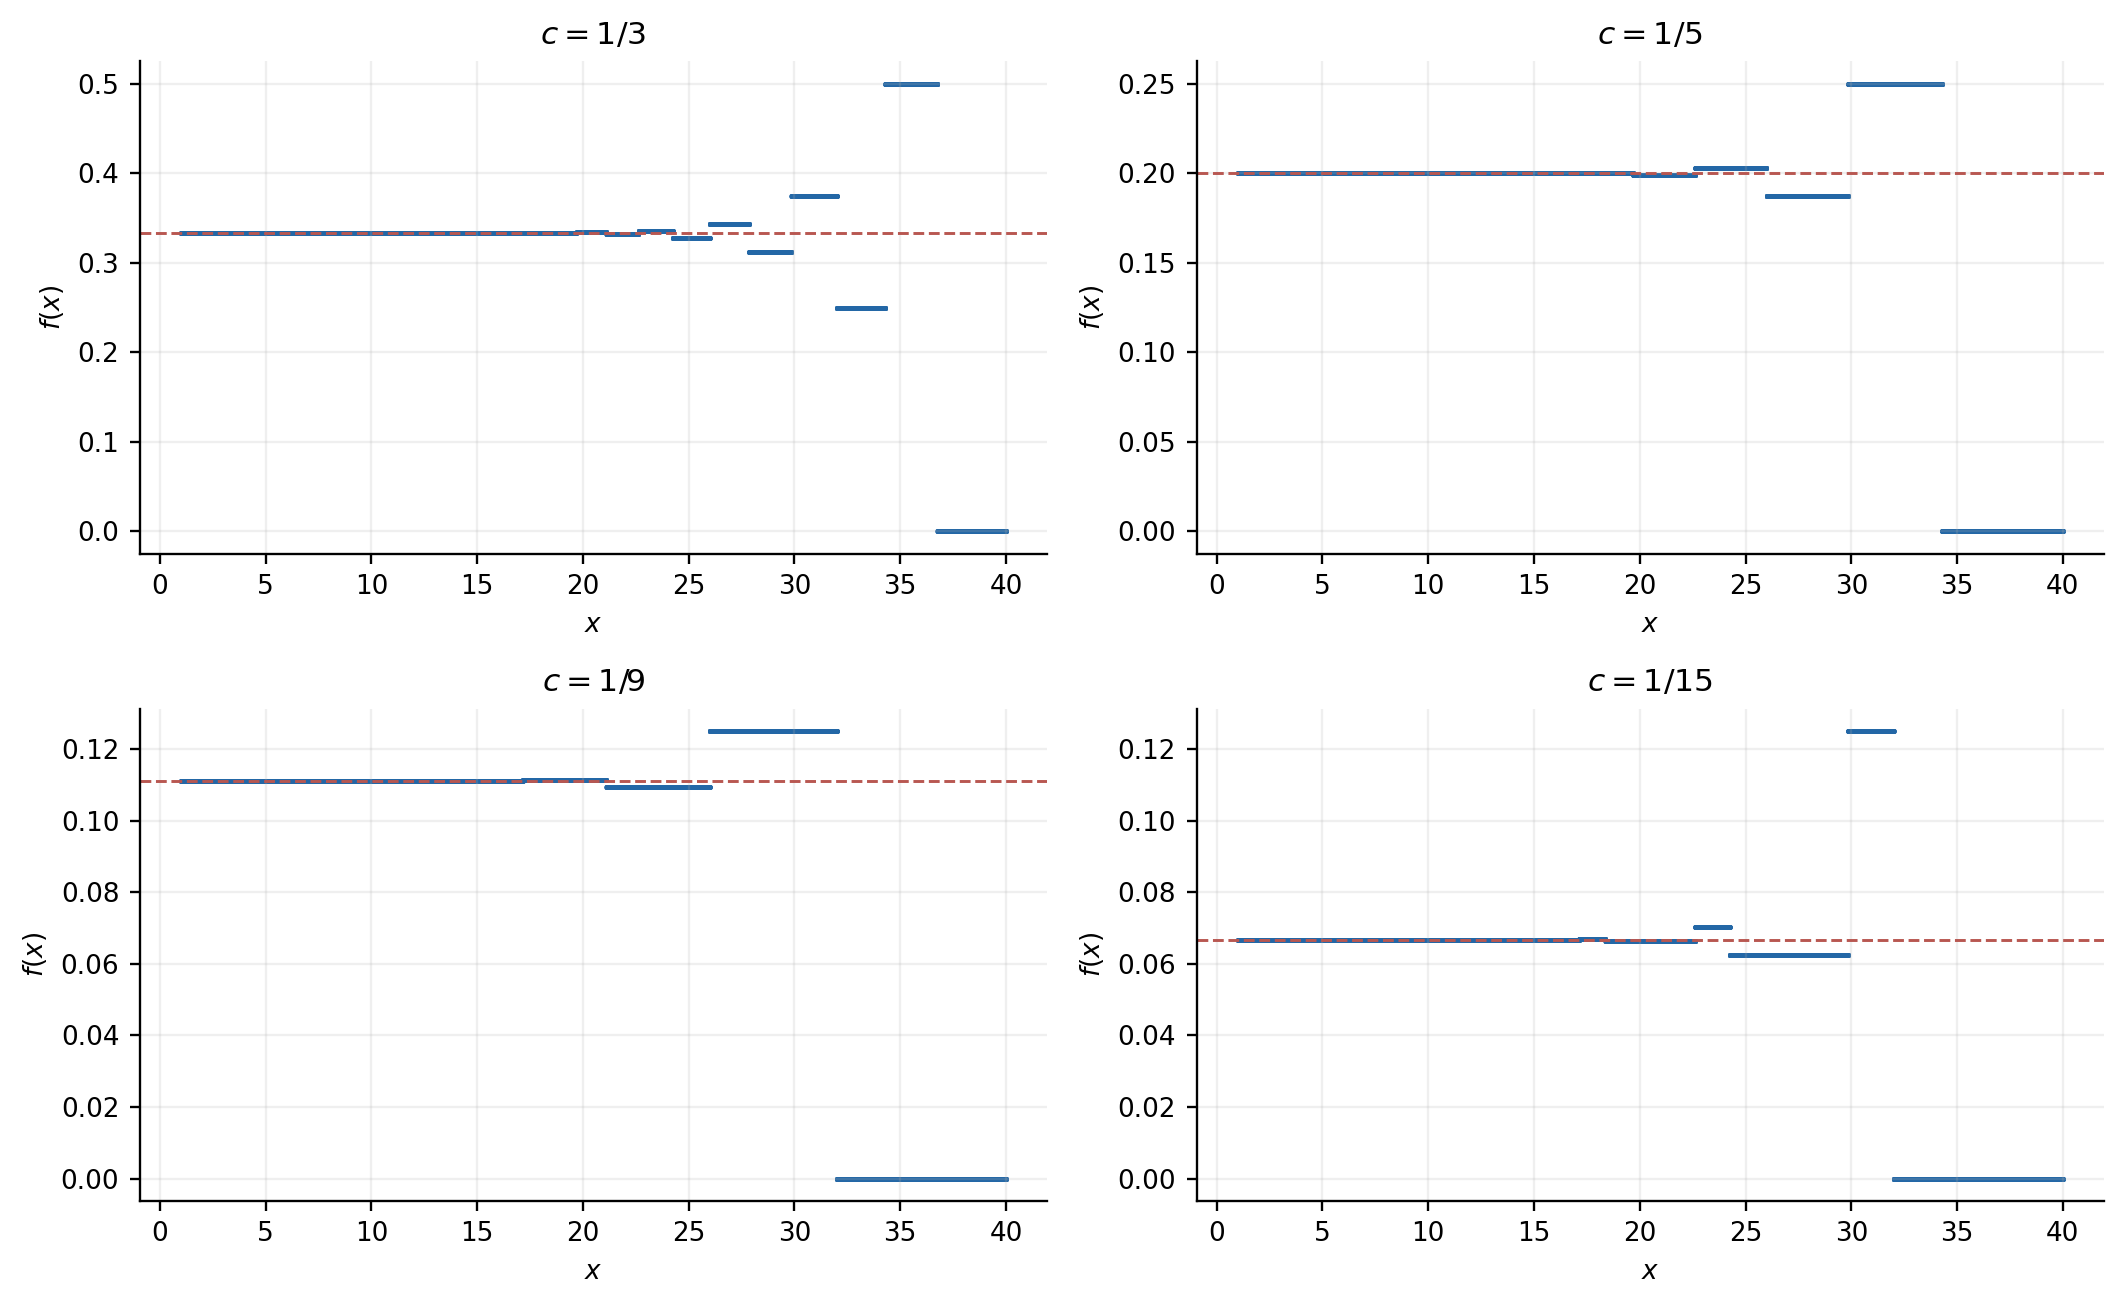
\includegraphics[width=.93\textwidth]{figs/09_reciprocal_odd_fractions.png}
\caption{Examples $c=1/d$ for selected odd denominators $d$ from the source's reciprocal-fraction Plotly experiment. The dashed line is the exact value $1/d$.}\label{fig:reciprocals}
\end{figure}

The supplied paper also reports relative errors for the stored approximations to $0.1$ and $1/3$ at selected binary64 inputs. Table~\ref{tab:relerr} reproduces these source measurements, with the convention that $(f-c)/c$ is measured relative to the \emph{stored} input $c$, not the ideal decimal constant. The relative error may be of order $10^{-9}$ at $x=5$, yet exceed $10^{-1}$ by $x=30$.

\begin{table}[htbp]
\centering
\caption{Relative errors $(f-c)/c$ reported in the source manuscript for binary64 fractions.}\label{tab:relerr}
\begin{tabular}{r rr}
\toprule
$x$ & $c=0.1$ &$c=1/3$\\
\midrule
$1$ & $+8.3\times10^{-16}$ &$-1.7\times10^{-16}$\\
$2$ & $-9.1\times10^{-13}$ &$-2.3\times10^{-13}$\\
$5$ & $-3.7\times10^{-9}$ &$+1.9\times10^{-9}$\\
$10$ & $+3.8\times10^{-6}$ &$+1.9\times10^{-6}$\\
$20$ & $-3.9\times10^{-3}$ &$+2.0\times10^{-3}$\\
$30$ & $+0.25$ &$+0.125$\\
$32.5$ & $-1$ &$-0.25$\\
\bottomrule
\end{tabular}
\end{table}

\section{Comparison between binary32 and binary64}
The same model applies to both IEEE 754 formats after replacing the precision $p$. For odd integers, the first affected $x$ decreases from approximately $39.40$ in binary64 to $5.28$ in binary32. The number $L$ of affected binades is unchanged for an exactly representable $c$ shared by both formats. For common non-dyadic literals, on the other hand, the binary32 approximation typically carries only about 24 relevant bits rather than about 53, and its predicted inexact interval is correspondingly narrower in log-space.

\begin{figure}[htbp]
\centering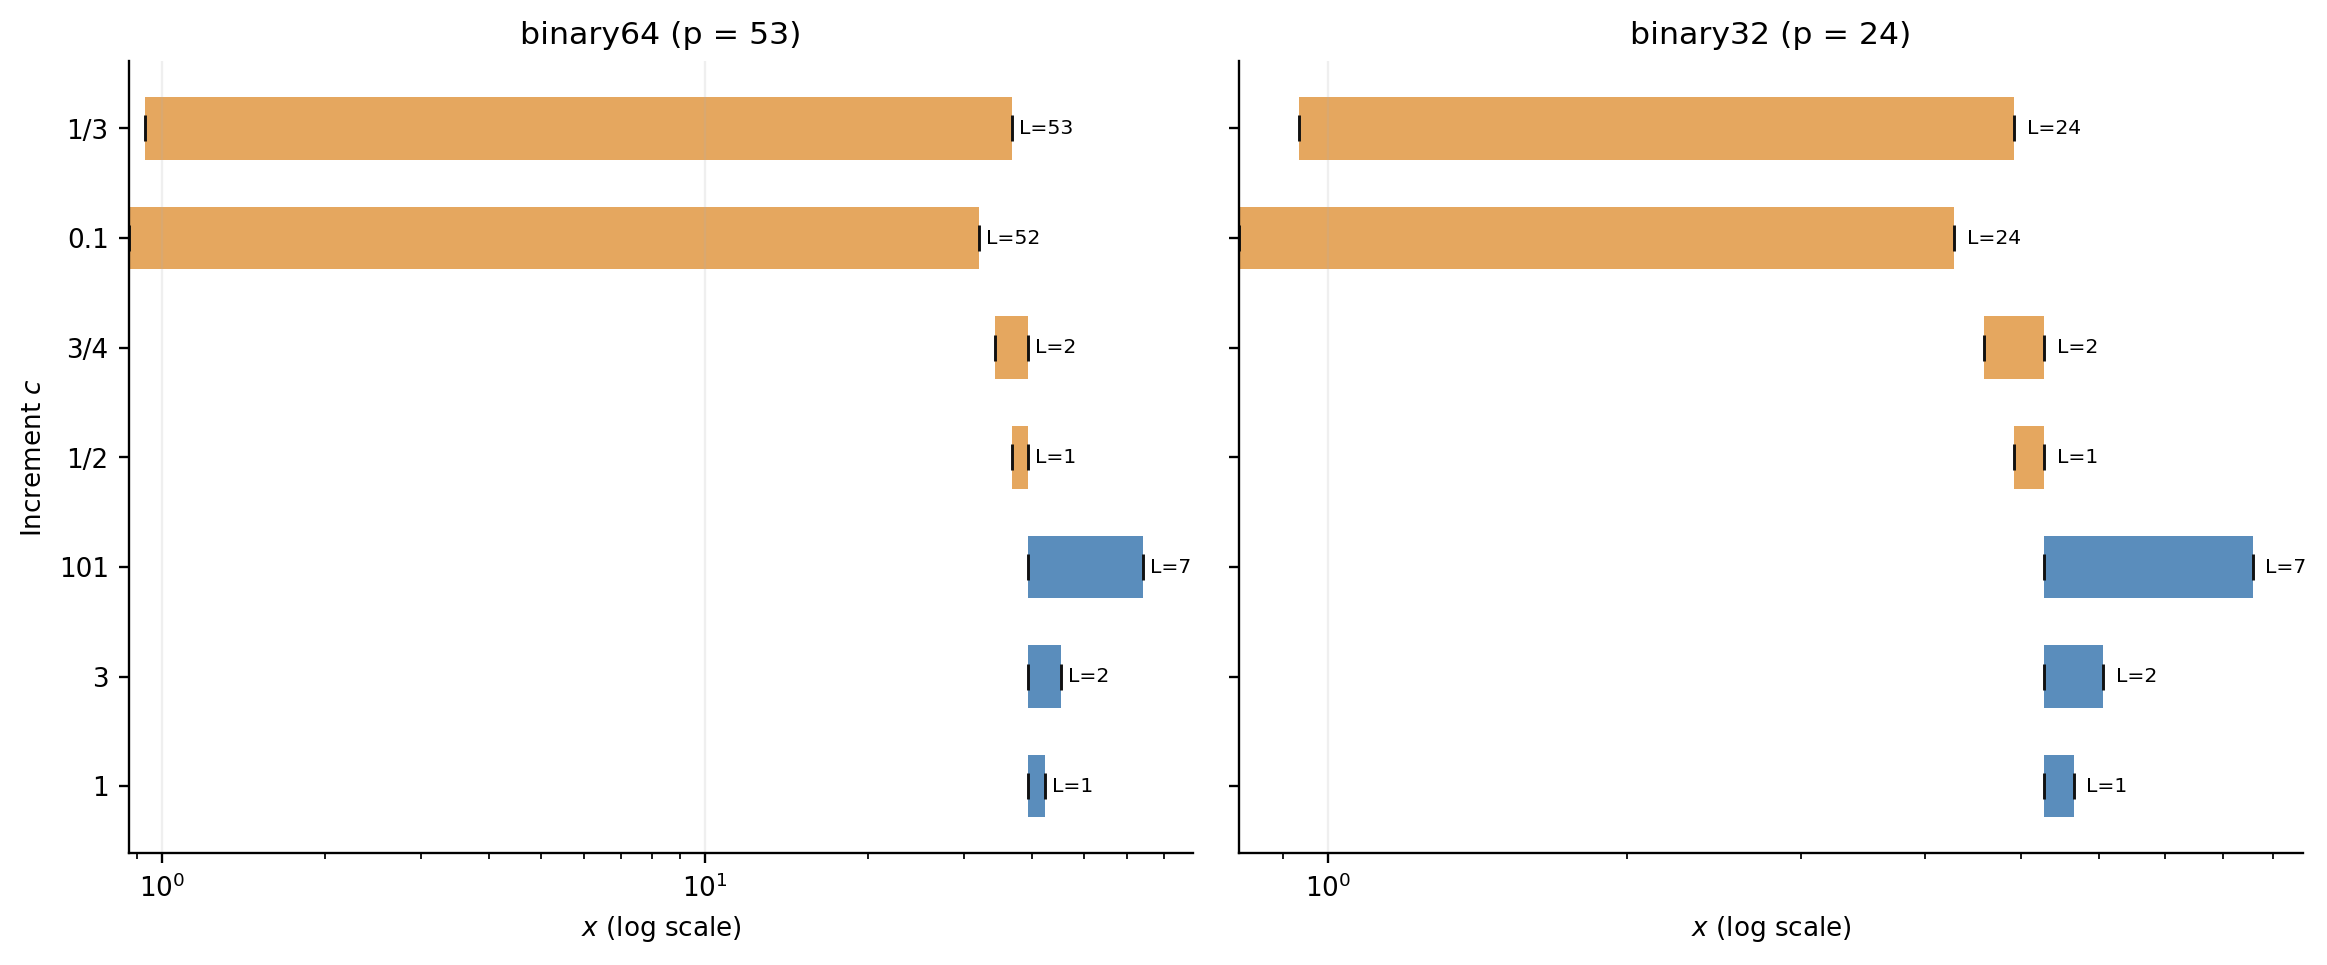
\includegraphics[width=.98\textwidth]{figs/07_precision_comparison.png}
\caption{Predicted inexact ranges in the two precisions for representative increments. The bars visualize the formulas for $x_1$ and $x_2$; they are not uncertainty intervals.}\label{fig:precision}
\end{figure}

The source study reports that the nearest-grid model matched its 1,611 tested increments in each precision after accounting for samples outside the model's domain (including binade crossings). These are reported outcomes from the original validation scripts. A particularly useful practical warning is that an input $c$ may itself change when converted to binary32; comparisons must therefore use the \emph{represented} $c$ in each format rather than assume that the same exact real increment is available to both.
